\begin{frame}{Centralisé}
    \begin{block}{Le centralisé offre\dots}
        \begin{itemize}
            \item Diversité d'acteurs.
            \item Accessibilité.
            \item Multiples fonctionnalités.
        \end{itemize}
    \end{block}
    \begin{block}{Mais\dots}
        \begin{itemize}
            \item Opacité des protocoles.
            \item Failles de sécurité.
            \item Collecte des données.
        \end{itemize}
    \end{block}
\end{frame}


\begin{frame}{Décentralisé}
    \begin{block}{Le décentralisé offre\dots\dots}
        \begin{itemize}
            \item Pas de tiers de confiance.
            \item Transparence.
            \item Fiabilité accrue.
        \end{itemize}
    \end{block}
    \begin{block}{Mais\dots}
        \begin{itemize}
            \item Difficiles d'accès.
            \item Intérêt économique faible.
        \end{itemize}
    \end{block}
\end{frame}

\begin{frame}{Conclusion générale}
    \begin{itemize}
        \item Flou entre centralisé/décentralisé.
        \item Définitions variables selon les plateformes.
        \item Grand nombre de projets mis à l'écart.
    \end{itemize}
\end{frame}

\begin{frame}{Conclusion générale - Tableau récapitulatif}
    \centering
    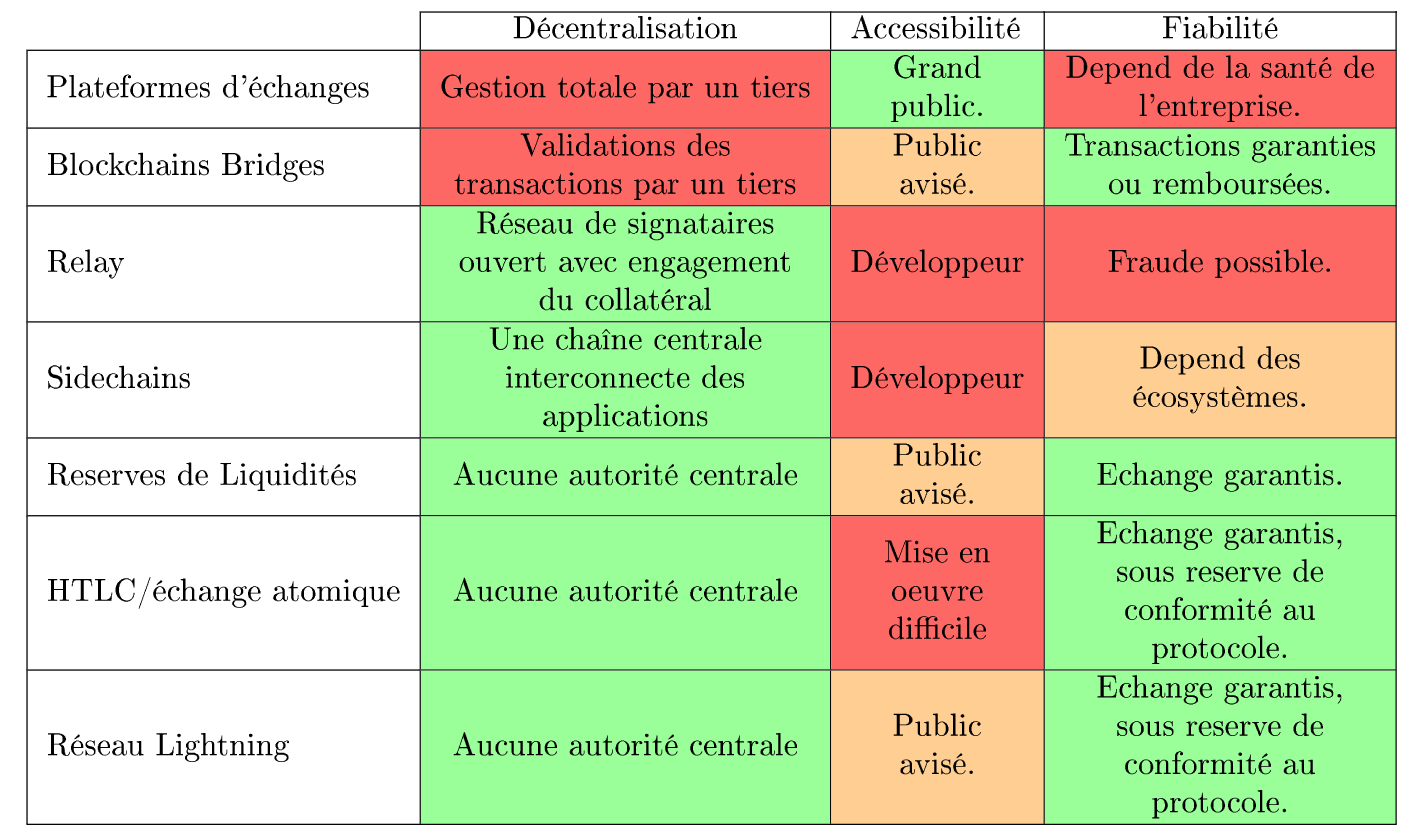
\includegraphics[scale = 0.3] {conclusion/tableau.png}
\end{frame}

\begin{frame}{Remerciements}
    \centering
    Merci de votre attention, n'hésitez pas à poser des questions.
\end{frame}

